

\chapter{Results}

In this chapter, we describe the results from our pose and depth experiments. In Chapter 3 we described an unsupervised pipeline for learning depth and visual odometry from monocular imagery. Similarly, in Chapter 4, adapted conventional 2D machine learning techniques to apply 4D image data to learning these tasks. Specifically, we recommended two variants of an algorithm for learning depth and visual odometry from light fields - the first uses all the information from the light field to generate a novel rendering of a single \textit{(U, V)} slice, while the second method uses the known configuration of the camera array to create a rendering of the complete light field. In this chapter, we contrast results for three algorithms - each of the two novel pipelines described in Chapter 4, and the existing monocular approach described in Chapter 3. For the two algorithms that we have suggested, we also evaluate three ingestion methods: focal-stacks, volumetric images, and tiled EPI images. 

First, we evaluate each algorithm's performance in pose-estimation, and demonstrate results for cumulated trajectories for several input-sequences. Subsequently, we'll evaluate the algorithms' performance in depth-prediction and photometric reconstruction. 

In each of our experiments, we use the same training dataset of ~9000 input images consisting of 48 short video-sequences. The testing set, which is also the same across all experiments, consists of ~400 input images over 4 video-sequences. 

\section{Pose Estimation and Visual Odometry}

An important metric of error that we use to evaluate pose prediction, is the \textit{absolute instantaneous error} for each of the 6 degrees-of-freedom that are estimated. This metric describes the magnitude of the error between the predicted and the true component. As described in Chapter 4, we have collected ground-truth pose data using a robotic manipulator platform with a repeatability of $\pm 0.01$ millimeters, thus allowing a strong evaluation of pose-estimation. Meanwhile, we can evaluate each pipeline's effectiveness in estimating the \textit{average cumulative error} by comparing the true trajectory with the predicted trajectory. 


\subsection{Single-view Reconstruction}

The following histograms summarise 400 observations of the absolute instantaneous error for each of the 6 degrees of freedom (translation and rotation in X, Y and Z), over three input methods (tiled epipolar images, focal stacks, and volumetric stacks).

\begin{figure}[H]
    \centering
    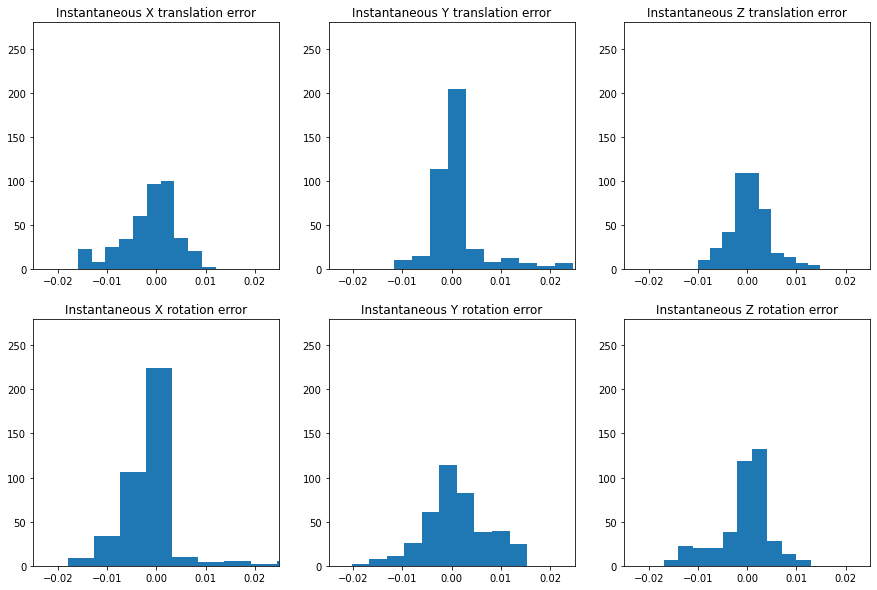
\includegraphics[width=\textwidth, height=3.35in]{images/result-examples/pose/errors/singlewarp-epi.png}
    \caption{Instantaneous absolute errors when \textbf{tiled epipolar images} are the input method.}
\end{figure}

\begin{figure}[H]
    \centering
    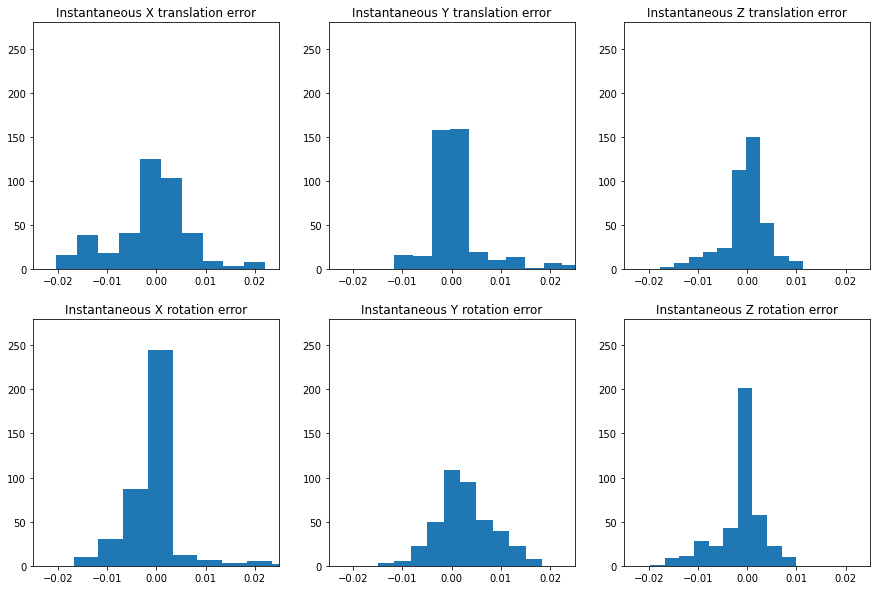
\includegraphics[width=\textwidth, height=3.35in]{images/result-examples/pose/errors/singlewarp-focalstack-17-5.png}
    \caption{Instantaneous absolute errors when \textbf{focal stacks} images are the input method.}
\end{figure}

\begin{figure}[H]
    \centering
    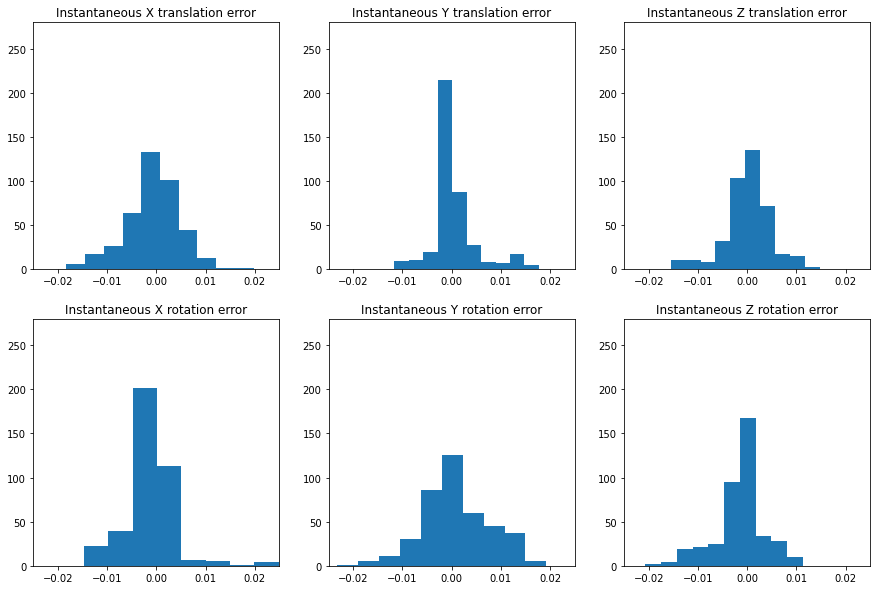
\includegraphics[width=\textwidth, height=3.35in]{images/result-examples/pose/errors/singlewarp-stack.png}
    \caption{Instantaneous absolute errors when \textbf{volumetric stacks} are the input method.}
\end{figure}

Figure 5.5 shows 2 examples of true and estimated trajectories for the three input methods. 

\begin{figure}[H]
    \subfloat[Tiled EPIs]{
        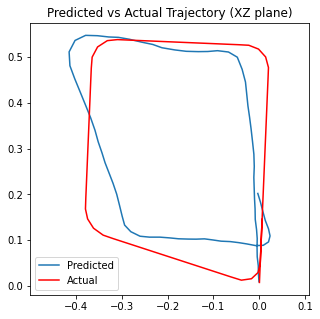
\includegraphics[height=1.9in]{images/result-examples/pose/trajectories/singlewarp/sw-epi-16.png}
    }
    \subfloat[Focal Stacks]{
        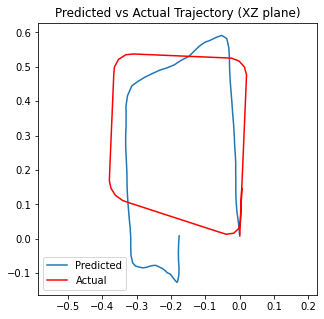
\includegraphics[height=1.9in]{images/result-examples/pose/trajectories/singlewarp/sw-focalstack-175-16.png}
    }
    \subfloat[Volumetric Images]{
        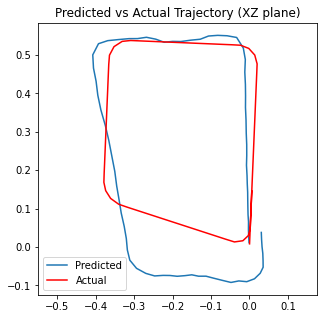
\includegraphics[height=1.9in]{images/result-examples/pose/trajectories/singlewarp/sw-stack-16.png}
    }\\
    \caption{Estimated and true trajectories for input sequence 16.}
    \setcounter{subfigure}{0}

    \subfloat[Tiled EPIs]{
        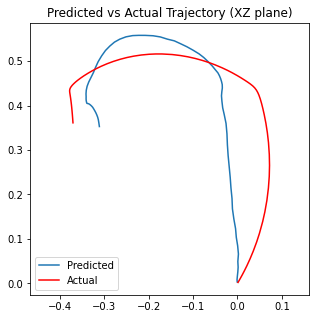
\includegraphics[height=1.9in]{images/result-examples/pose/trajectories/singlewarp/sw-epi-44.png}
    }
    \subfloat[Focal Stacks]{
        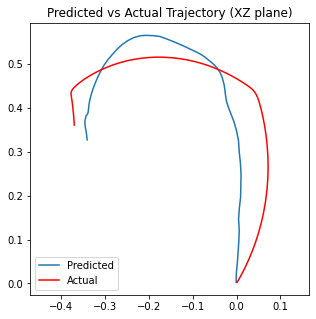
\includegraphics[height=1.9in]{images/result-examples/pose/trajectories/singlewarp/sw-focalstack-175-44.png}
    }
    \subfloat[Volumetric Images]{
        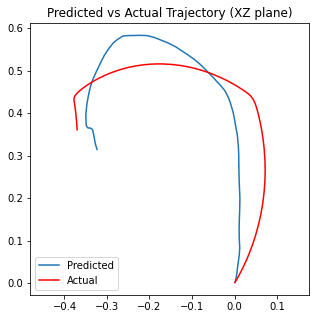
\includegraphics[height=1.9in]{images/result-examples/pose/trajectories/singlewarp/sw-stack-44.png}
    }
    \caption{Estimated and true trajectories for input sequence 44.}
    \setcounter{subfigure}{0}
\end{figure}

Table 5.1 summarises the instatnaneous and cumulative errors for the three input methods. 
 
\begin{table}[htbp]
    \caption{Mean Absolute Instantaneous Error and Cumulative Error}
    \centering
    \begin{tabular}{@{}lll@{}}
        \toprule
        Input Method        & Absolute Instantaneous Error   & Cumulative Error  \\
        \midrule 
        Tiled EPI Polar Images & TODO & TODO \\
        Focal Stacks & TODO & TODO \\
        Volumetric Stacks & TODO & TODO \\
        \bottomrule
        
    \end{tabular}
\end{table}


\subsection{Light field Reconstruction}

Here we describe the performance of the second variant of our suggested pipeline, using the known camera configuration to photometrically warp the complete light field. Because this pipeline incorporates known information about the relationship between individual sub-apertures on the camera module, we expect this pipeline to show improved performance in pose estimation and demonstrate improved scale-consistency.

We carry this expectation because this variant of the pipeline generates a stronger supervision signal due to the significantly larger number of pixels used to compute the photometric warp error. Furthermore, this variant penalises small errors in the pose-estimate significantly more heavily than in the previous variant. 

\begin{figure}[H]
    \centering
    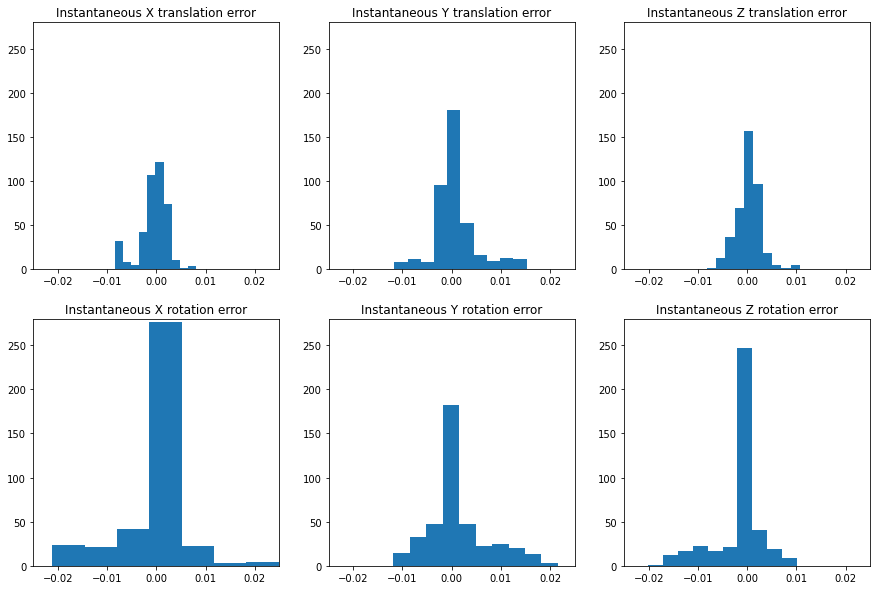
\includegraphics[width=\textwidth, height=3.2in]{images/result-examples/pose/errors/multiwarp-epi.png}
    \caption{Histograms of instantaneous absolute error for each of the 6 degrees of freedom estimated by our pose network when epipolar images are the input method.}
\end{figure}
\begin{figure}[H]
    \centering
    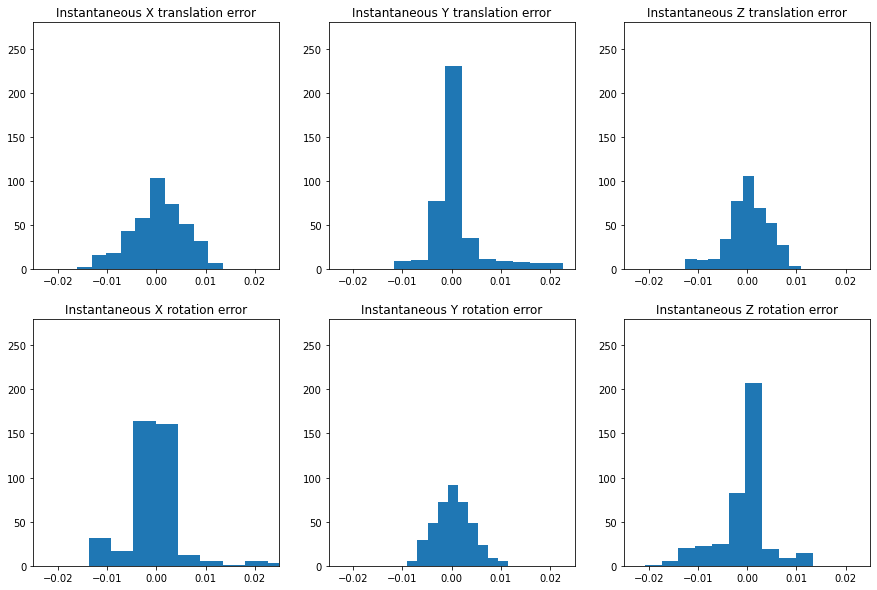
\includegraphics[width=\textwidth, height=3.2in]{images/result-examples/pose/errors/multiwarp-focalstack-17-5.png}
    \caption{Histograms of instantaneous absolute error for each of the 6 degrees of freedom estimated by our pose network when focal stacks are the input method.}
\end{figure}
\begin{figure}[H]
    \centering
    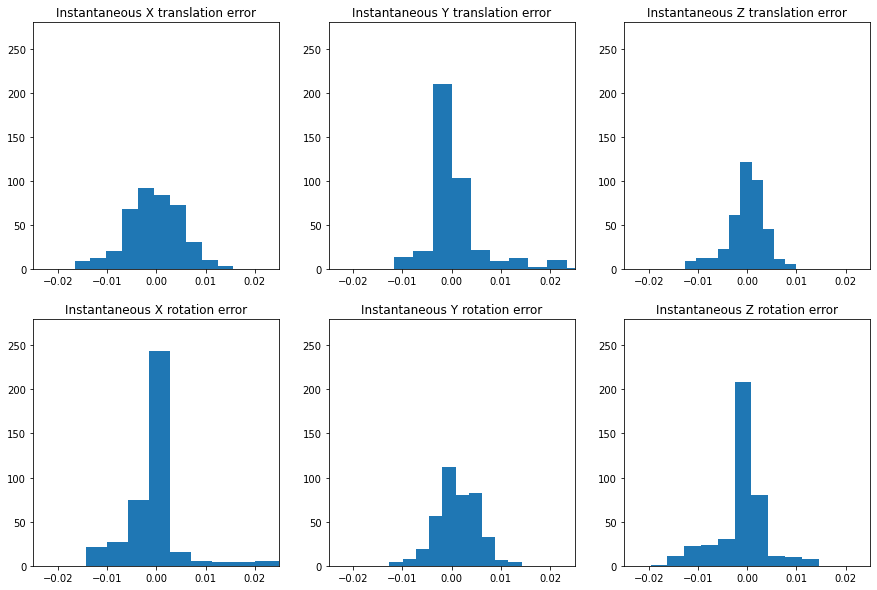
\includegraphics[width=\textwidth, height=3.2in]{images/result-examples/pose/errors/multiwarp-stack.png}
    \caption{Histograms of instantaneous absolute error for each of the 6 degrees of freedom estimated by our pose network when volumetric images are the input method.}
\end{figure}



\begin{figure}[H]
    \subfloat[Tiled EPIs]{
        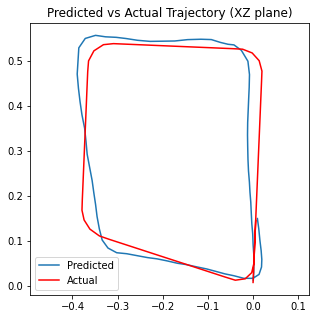
\includegraphics[height=2in]{images/result-examples/pose/trajectories/multiwarp/mw-epi-16.png}
    }
    \subfloat[Focal Stacks]{
        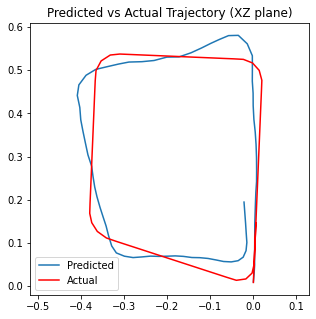
\includegraphics[height=2in]{images/result-examples/pose/trajectories/multiwarp/mw-fs-175-16.png}
    }
    \subfloat[Volumetric Images]{
        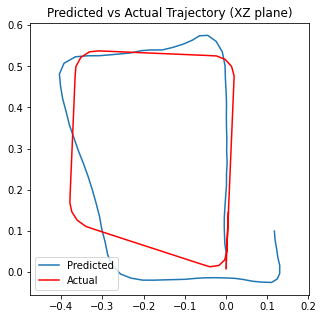
\includegraphics[height=2in]{images/result-examples/pose/trajectories/multiwarp/mw-stack-16.png}
    }
    \caption{Estimated and true trajectories for input sequence 16.}
    \setcounter{subfigure}{0}
    \subfloat[Tiled EPIs]{
        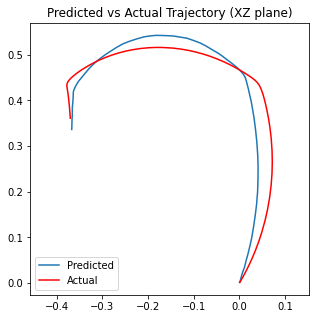
\includegraphics[height=2in]{images/result-examples/pose/trajectories/multiwarp/mw-epi-44.png}
    }
    \subfloat[Focal Stacks]{
        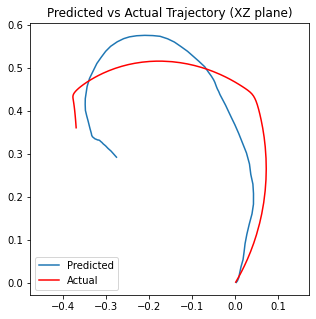
\includegraphics[height=2in]{images/result-examples/pose/trajectories/multiwarp/mw-fs-175-44.png}
    }
    \subfloat[Volumetric Images]{
        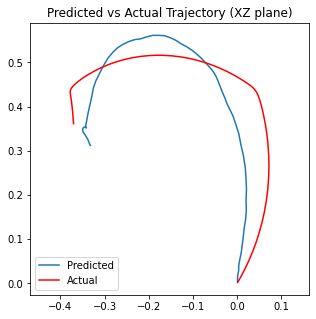
\includegraphics[height=2in]{images/result-examples/pose/trajectories/multiwarp/mw-stack-44.png}
    }
    \caption{Estimated and true trajectories for input sequence 44.}
    \setcounter{subfigure}{0}
\end{figure}

\begin{table}[htbp]
    \caption{Mean Absolute Instantaneous Error and Cumulative Error}
    \centering
    \begin{tabular}{@{}lll@{}}
        \toprule
        Input Method        & Absolute Instantaneous Error   & Cumulative Error  \\
        \midrule 
        Tiled EPI Polar Images & TODO & TODO \\
        Focal Stacks & TODO & TODO \\
        Volumetric Stacks & TODO & TODO \\
        \bottomrule
        
    \end{tabular}
\end{table}


\subsection{Monocular Approach}

\begin{figure}[H]
    \subfloat[Sequence 16]{
        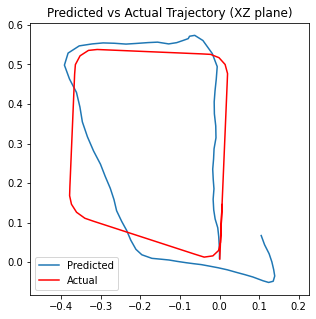
\includegraphics[height=3in]{images/result-examples/pose/trajectories/monocular/monocular-16.png}
    }
    \subfloat[Sequence 44]{
        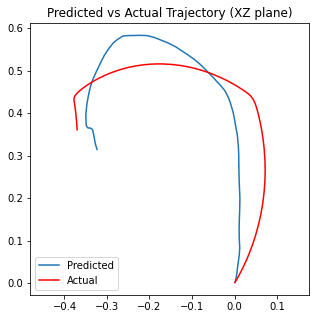
\includegraphics[height=3in]{images/result-examples/pose/trajectories/monocular/monocular-44.png}
    }
    \caption{Estimated and true trajectories using monocular imagery.}
    \setcounter{subfigure}{0}
\end{figure}



\subsection{Comparison between Pipelines and Summary}

\section{Depth and Photometric Reconstruction}

\subsection{Single-view Reconstruction}
\subsection{Light field Reconstruction}
\subsection{Monocular Approach}

\subsection{Comparison between Pipelines and Summary}





